%\documentclass[trans,handout]{beamer}
\documentclass[trans]{beamer}

%\usepackage{pgfpages}
%\pgfpagesuselayout{4 on 1}[a4paper,landscape,border shrink=5mm]
%\pgfpagesuselayout{2 on 1}[a4paper,border shrink=5mm]

\usepackage[utf8]{inputenc}
\usepackage{graphicx}
\usepackage{multicol}
\usepackage{xcolor}
\usepackage{listings}
\lstset{frame=tb,
  aboveskip=3mm,
  belowskip=3mm,
  showstringspaces=false,
  columns=flexible,
  basicstyle={\small\ttfamily},
  numbers=none,
  numberstyle=\tiny\color{gray},
  keywordstyle=\color{blue},
  commentstyle=\color{green!55!blue},
  stringstyle=\color{purple},
  breaklines=true,
  breakatwhitespace=true,
  tabsize=4
}
\usepackage{hyperref}
\hypersetup{
  colorlinks=true,
  linkcolor=black,
  urlcolor=blue
}
\graphicspath{{figures/}}

% for the logo slide; source: https://tex.stackexchange.com/questions/7925/big-arrows-between-images
\def\Arrow{\raisebox{-.5\height}{\scalebox{4}{$\rightarrow$}}}
\def\Image#1{\raisebox{-.5\height}{\includegraphics[width=3.5cm]{#1}}}

\newcommand\Wider[2][3em]{%
\makebox[\linewidth][c]{%
  \begin{minipage}{\dimexpr\textwidth+#1\relax}
  \raggedright#2
  \end{minipage}%
  }%
}

\title{
  
\includegraphics[height=.3\textwidth]{figures/biopython_logo_s.png}\\[1em]
  Biopython Project Update 2017}
\subtitle{}
\author[Sourav Singh]{
  \textbf{Sourav Singh}, Christian Brueffer, Peter Cock,\\
  and the Biopython Contributors}
\institute[Savitribai Phule Pune University]{Savitribai Phule Pune University\\
  India\\[1em]
  Bioinformatics Open Source Conference 2017, Prague, CZ \\[1em]
}
\date{July 23th, 2017}

\setcounter{tocdepth}{2}
\setbeamertemplate{caption}{\insertcaption}


% ToC at the beginning of every section
%\AtBeginSection[]
%{
 % \begin{frame} % with <beamer> => doesn't appear in handout mode
  %  \frametitle{Outline} %% Put the title you want, or none!
  %  \tableofcontents[currentsection,currentsection]
 % \end{frame}
%}

\begin{document}
\maketitle

\section{The Biopython Project}
\frame
{
  \frametitle{What is Biopython?}

  \begin{itemize}
  \item Collection of modules for biological computation in Python
  \begin{itemize}
  \item Sequence handling and motifs, parsers, database queries, protein structures, phylogenetics, tool wrappers and more.
  \end{itemize}
  \item Started in 1999, first release in 2000
  \item Open source and freely available (Biopython license)
  \end{itemize}

  \begin{center}
  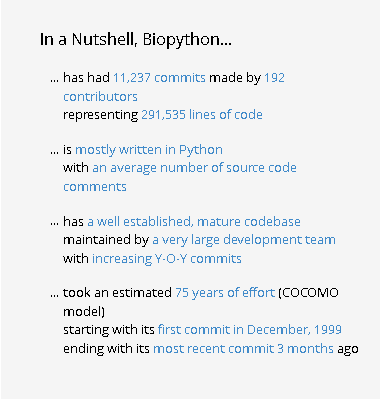
\includegraphics[width=0.4\textwidth]{figures/openhub-bp-nutshell.png}
  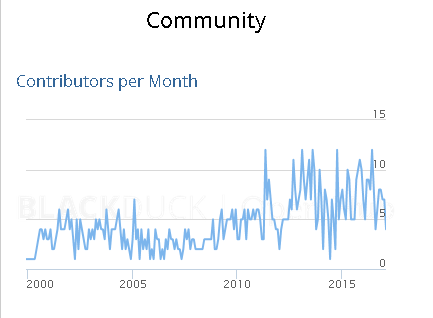
\includegraphics[width=0.5\textwidth]{figures/openhub-bp-community-activity.png}
  \end{center}
  \small{Source: \url{https://www.openhub.net/p/biopython}}
}
\frame
{
  \frametitle{80 named contributors this year, 51 newcomers with star!}
  \Wider{
  \tiny{
  \begin{multicols}{4}
  \begin{itemize}
  \item Aaron Kitzmiller*
  \item Aaron Rosenfeld
  \item Adam Kurkiewicz*
  \item Adam Novak*
  \item Adil Iqbal*
  \item Adrian Altenhoff*
  \item Allis Tauri*
  \item Andrew Dalke
  \item Andrew Guy*
  \item Andrew Sczesnak*
  \item Anthony Bradley*
  \item Ariel Aptekmann*
  \item Ben Fulton
  \item Bernhard Thiel*
  \item Bertrand Caron*
  \item Bertrand N{\'e}ron % Bertrand N�ron
  \item Blaise Li*
  \item Brandon Carter*
  \item Brandon Invergo
  \item Carlos Pena
  \item Carlos R{\'i}os % Carlos R�os
  \item Chris Rands
  \item Chris Warth
  \item Connor T. Skennerton
  \item Emmanuel Noutahi
  \item Eric Rasche
  \item Eric Talevich
  \item Foen Peng*
  \item Francesco Gastaldello*
  \item Francisco Pina-Martins*
  \item Fran{\c c}ois Coste* % Fran�ois Coste
  \item Frederic Sapet*
  \item Hector Martinez*
  \item Iddo Friedberg
  \item Jacek {\'S}mieta{\'n}ski % Jacek ?mieta?ski
  \item Jack Twilley*
  \item Jared Andrews*
  \item Jeroen Van Goey*
  \item Jimmy O'Donnell*
  \item John Kern*
  \item Jordan Willis*
  \item Joshua Meyers*
  \item Jo{\~a}o Rodrigues % Jo�o Rodrigues
  \item Kai Blin
  \item Kristian Davidsen*
  \item Kurt Graff*
  \item Lenna Peterson
  \item Leonhard Heizinger*
  \item Marcin Magnus*
  \item Markus Piotrowski
  \item Mateusz Korycinski*
  \item Maximilian Greil*
  \item Micha{\l} J. Gajda* % Micha? J. Gajda*
  \item Michiel de Hoon
  \item Milind Luthra*
  \item morrme*
  \item Noam Kremen*
  \item Olivier Morelle*
  \item Oscar G. Garcia*
  \item Owen Solberg
  \item Patrick Kunzmann*
  \item Peter Cock
  \item Rasmus Fonseca*
  \item Richard Neher*
  \item Rodrigo Dorantes-Gilardi*
  \item Sacha Laurent*
  \item Sebastian Bassi
  \item Sourav Singh*
  \item Spencer Bliven*
  \item Stefans Mezulis
  \item Steve Bond
  \item Steve Marshall*
  \item Ted Cybulski*
  \item Tiago Antao
  \item Travis Wrightsman
  \item Uri Laserson
  \item Uwe Schmitt*
  \item Veronika Berman*
  \item Vincent Davis
  \item Wibowo Arindrarto % Wibowo `Bow' Arindrarto
  \item Xiaoyu Zhuo*
  \item Zheng Ruan
  \end{itemize}
  \end{multicols}
  }
  }
}

%%%%%%%%%%%%%%%%%%%%%%%%%%%%%%%%%%%%%%%%%%%%%%%%%%%%%%%%%%%%%%%%%%%%%%%%%%%%%%%%

\section{New Releases and Beyond}
\frame
{
\center{\LARGE Biopython 1.68 (released 2016-08-25)}
}
\frame
{
  \frametitle{New Features in Biopython 1.68}

  \begin{itemize}
  \item Final Release supporting Python 2.6
  \item \texttt{Bio.PDB} can now parse the new MMTF format.
  \item \texttt{Bio.pairwise2} rewritten to address speed and problems with local alignments.
  \item \texttt{SeqGui} and \texttt{xbbtools} rewritten using tkinter.
  \item Biopython now uses HTTPS instead of HTTP to connect to NCBI Entrez and QBLAST API.
  \end{itemize}

}
\frame
{
  \center{\LARGE Biopython 1.69 (released 2017-04-06)}
}
\frame
{
  \frametitle{Start of re-licensing plan}

  \begin{itemize}
  \item Biopython 1.69 marked start of our re-licensing plan.
  \item transitioning away from liberal \emph{Biopython License Agreement},
  to the widely used \emph{3-Clause BSD License}.
  \item Code base authorship being reviewed file-by-file,
  \item will gradually dual license the entire project.
  \end{itemize}

}
\frame
{
  \frametitle{New features in Biopython 1.69}
  \begin{itemize}
  \item Improved PyPy support, all NumPy and most C code works.
  \item Cellosaurus cell line database, cell ontologies and catalogues accessible through the \texttt{Bio.ExPASy} module.
  \item MAF files supported in \texttt{Bio.AlignIO}, including indexing.
  \item \texttt{Bio.Restriction} updated to REBASE Feb 2017 enzyme list
  \item \texttt{Bio.PDB} can download PDBx/mmCif (new default), PDB (old default), PDBML/XML, and MMTF protein structures.
  \item \texttt{Bio.Affy} supports version 4 of Affymetrix CEL format.
  \end{itemize}

}

\frame
{
  \center{\LARGE Biopython 1.70 (released 2017-07-10)}
}

\frame
{
  \frametitle{New logo for Biopython}

  \begin{itemize}
  \item Version 1.70 marks the transition towards a new logo for Biopython.

  \Image{figures/biopython.jpg}\hspace{1em}\Arrow\hspace{1em}
  \Image{figures/biopython_logo_s.png}

  \item The new logo was created by Patrick Kunzmann in 2017 and had support from the Python Software Foundation and the Biopython developers community.
  \end{itemize}

}

\frame
{
  \frametitle{New features in Biopython 1.70}

  \begin{itemize}
  \item Module \texttt{Bio.AlignIO}
  \begin{itemize}
  \item Support for XMFA file format using \texttt{Bio.AlignIO.MauveIO}
  \end{itemize}
  \end{itemize}
  \begin{itemize}
  \item Module \texttt{Bio.SearchIO}
  \begin{itemize}
  \item Support for new arguments to read and write blast-xml files.
  \end{itemize}
  \item Deprecate \texttt{Bio.GA} and \texttt{Bio.NeuralNetwork} modules.
  \item Deprecate support for Jython.
  \item Dropped support for Python 3.3
  \end{itemize}

}

\frame
{
  \frametitle{Currently supported Python versions}

  \begin{itemize}
  \item Python 2.7
  \item Python 3.4
  \item Python 3.5
  \item Python 3.6
  \item PyPy 5.7
  \item PyPy3 5.8 beta
  \item Jython 2.7 (support is deprecated)
  \end{itemize}
}

\section{General Updates}

\frame
{
  \frametitle{On going work}

  \begin{itemize}
  \item Miscellaneous bug fixes
  \item Improving built-in docstrings (Python API documentation)
  \item Test suite enhancements and coverage improvements
  \item Better \href{https://www.python.org/dev/peps/pep-0008/}{PEP8} and \href{https://www.python.org/dev/peps/pep-0257/}{PEP257} coding style adherence
  \item Automating build process for wheel packages \url{http://github.com/biopython/biopython-wheels}
  \end{itemize}
}

\frame
{
  \frametitle{Continuous Integration}

  \begin{itemize}
  \item TravisCI
      \begin{itemize}
      \item Linux testing with coverage
      \item Style checks with flake8
      \item Experimenting with Build Stages
      \end{itemize}
  \item Appveyor (Windows testing with coverage)
  \item Codecov.io (tracking unit test coverage)
  \item Quantified Code (code metrics etc, sadly shutting down)
  \item Landscape.io (``health score'')
  \end{itemize}

  \begin{columns}
  \column{0.4\textwidth}
  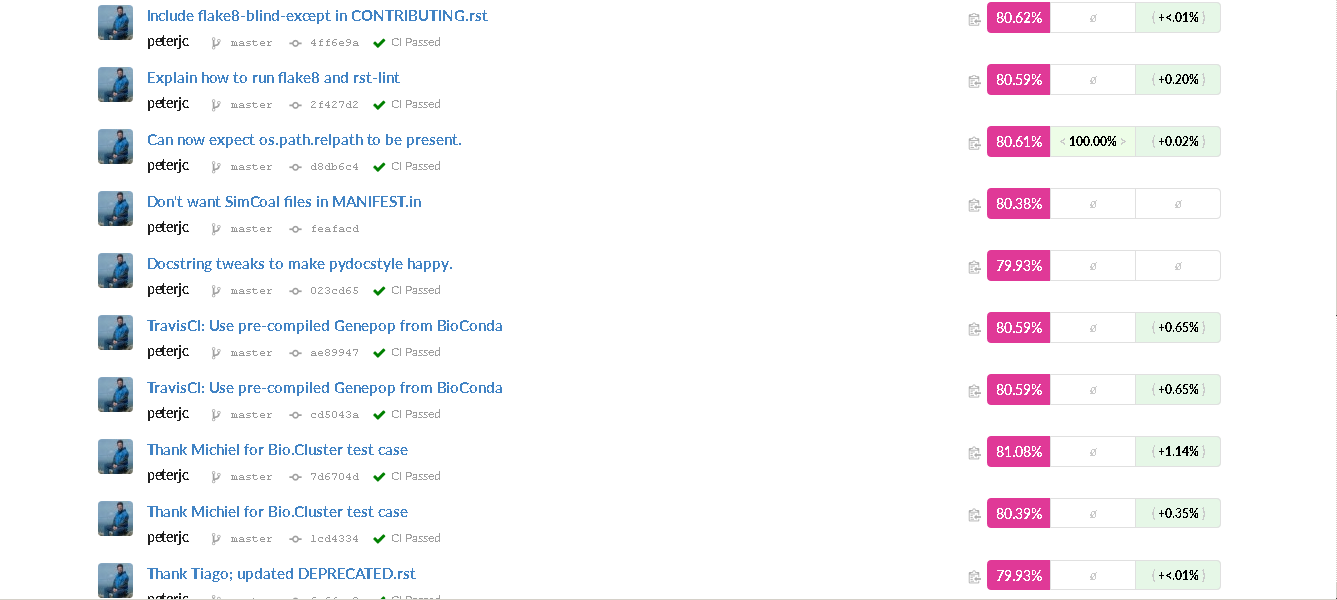
\includegraphics[width=1\textwidth]{figures/bp-codecov.png}
  \column{0.6\textwidth}
  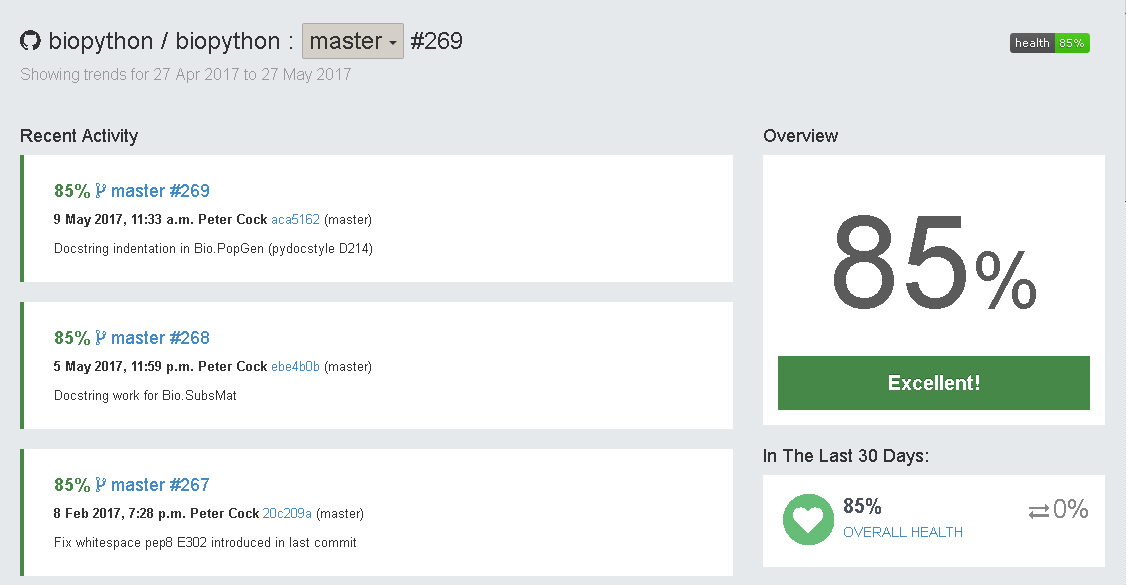
\includegraphics[width=1\textwidth]{figures/bp-landscape.png}
  \end{columns}
}

\section{Conclusion}
\frame
{
  \frametitle{Conclusion}

  \begin{itemize}
  \item Lots of new contributors
  \item Turning new contributors into recurring ones
  \item Lots of new stuff
  \item Lots more automation with Continuous Integration services
  \item Biopython 1.71 in the near future
  \end{itemize}
}

\frame
{
  \frametitle{Acknowledgements}

  \begin{minipage}{1\textwidth}
  \begin{columns}
  \column{0.5\textwidth}
  \begin{itemize}
  \item Peter Cock
  \item Biopython Community
  \end{itemize}
  \column{0.5\textwidth}
  
\includegraphics[width=0.7\textwidth]{figures/biopython_logo_s.png}
  \end{columns}
  \end{minipage}

  \vspace{1.0cm}

  \begin{minipage}{1\textwidth}
  \begin{columns}
  \column{0.4\textwidth}
  \href{https://github.com/biopython/}{
\includegraphics[width=0.9\textwidth]{figures/github-logo.jpg}}\\
  \href{https://travis-ci.org/biopython/biopython/branches}{
\includegraphics[width=0.9\textwidth]{figures/travisci-logo.png}}\\
  \href{https://landscape.io/github/biopython/biopython}{
\includegraphics[width=0.9\textwidth]{figures/landscape.png}}\\
  \column{0.25\textwidth}
  \href{https://ci.appveyor.com/project/biopython/biopython/history}{
\includegraphics[width=0.8\textwidth]{figures/appveyor-logo-256.png}}\\
  \quad\\
  \href{https://codecov.io/github/biopython/biopython/}{
\includegraphics[width=0.8\textwidth]{figures/codecov-logo.png}}\\
  \column{0.25\textwidth}
  \href{https://www.quantifiedcode.com/app/project/gh:biopython:biopython/}{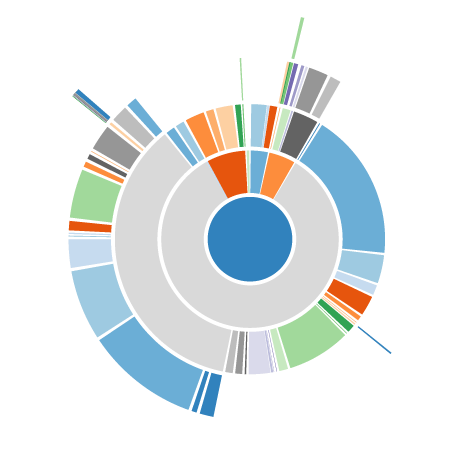
\includegraphics[width=0.9\textwidth]{figures/quantifiedcode-logo.png}}\\
  \href{https://www.open-bio.org/}{
\includegraphics[width=0.9\textwidth]{figures/obf-logo.png}}\\
  \end{columns}
  \end{minipage}
}

\section*{Acknowledgements}
\frame
{
  \frametitle{Resources!}

  %\begin{center}
  Website:\\
  \begin{itemize}
  \item \url{http://biopython.org}
  \end{itemize}

  Repositories:\\
  \begin{itemize}
  \item Main: \url{http://github.com/biopython/biopython}
  \item Website: \url{https://github.com/biopython/biopython.github.io}
  \end{itemize}

  Mailing lists:
  \begin{itemize}
  \item General list: \url{biopython@biopython.org}
  \item Developers list: \url{biopython-dev@biopython.org}
  \end{itemize}

  Biostars:
  \begin{itemize}
  \item \url{https://www.biostars.org/t/biopython/} (``biopython'' category)
  \end{itemize}
  %\end{center}
}

\end{document}
